\subsubsection{Merge Sort}

Figure \ref{fig:native_merge_sort} illustrates the time it takes for each language to sort one million randomly generated positive integers in ascending order. Note the severe difference in performance for Python.

\begin{figure}[h]
	\centering
	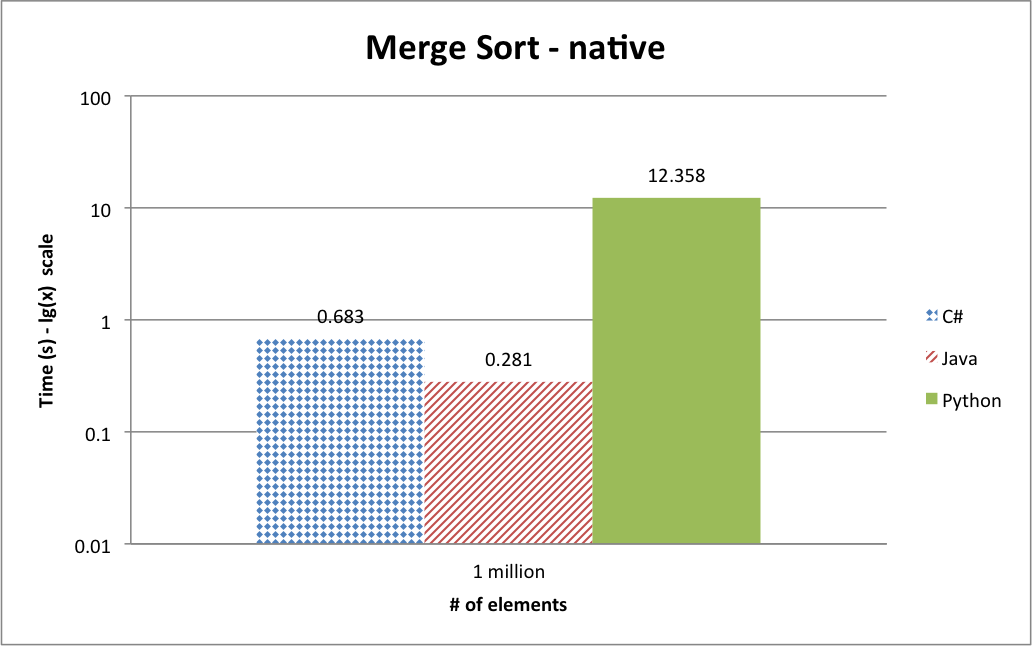
\includegraphics[width=1.0\linewidth]{chapters/new_media/MergeSortNative.png}
	\caption{This test uses the Merge sort algorithm to sort one million elements in ascending order. Lower is better. Note that the vertical axis is base 10 logarithmic. Java was the fastest with 0.281 seconds while Python was the slowest with 12.358 seconds.}
	\label{fig:native_merge_sort}
\end{figure}
